\chapter{Introduction to GEANT4}
\label{chap:G4Intro}
GEANT4 is a free toolkit for the simulation of particles as they travel through matter.
While nothing can replace the \href{http://geant4.web.cern.ch/geant4/G4UsersDocuments/UsersGuides/ForApplicationDeveloper/html/index.html}{User's Manual}, this is intended as a short guide to introduce a reader to the GEANT4 toolkit, and provide background on how the simulations were implemented.

\section{Toolkit Fundamentals}
A simulation in the GEANT4 toolkit requires a detector geometry (including materials), particles and interactions, and primary events.
Once the geometry and physics has been described, GEANT4 then tracks the primary particle (and generated secondaries) until the particle leaves the world volume, slows down to zero kinetic energy, or disappears by an interaction or decay. 
Particles can also be killed by implementing a range a cut, in which the particle is killed once its energy is less than the range.
The GEANT4 toolkit employs the following notation to describe a simulation.
A \textit{track} contains information about the a particles steps through a material, and acts like a snapshot of the particle.
\textit{Processes} contain implementations of models of the physics interactions.
Processes are used by \textit{tracking}, which can be thought of a linked list of tracks, where the links between the tracks are the processes.
A collection of tracking objects then makes up an \textit{event}.
A \textit{run} is then events that share a common beam and detector implementation.
A description of a run in GEANT4 is as follows.
At the beginning of a run the geometry is optimized and cross-sections are computed for the materials involved in the run.
Primary particles are then generated, and the corresponding tracks are then pushed into an event stack.
Each track in the stack is then processed until the event stack is empty.
Tracks that are above the cutoff value and inside the world geometry are processed by the use of a \textit{step} (a change in the track) and then pushed back onto the track.

\section{Optional User Classes}
Access to the simulation results is then provided by UserAction classes.
These classes are employed to hook into the GEANT4 simulation internals.
The user classes used in these simulations are described below.
\begin{itemize}
  \item \verb+G4UserRunAction+ - which has methods that are called before the beginning of each run and at the end of each run. Typical usage is to initialize histograms and book them at then end of the run.
  \item \verb+G4UserEventAction+ - has methods that are called before and after each event. Typically it is used for summarizing an event, such as calculating the total energy deposition or track length.
  \item \verb+G4UserStackingAction+ - this class is called before each track is pushed onto the event stack, and provides an opportunity for the user to kill tracks.
\end{itemize}
It should be noted that if a track is killed in the stacking or tracking action that GEANT4 does account for the lost energy in the track, thus the user is responsible for recording it if it is desired.

\section{Physics List}
The physics list in GEANT4 describe how the particle interact with matter.
There are seven major categories of physics that are considered in GEANT4; electromagnetic, hadronic, transportation, decay, optical, photolepton \& hadron, and parameterisation.
A physics process is applied to particle in GEANT4 after polling all of the processes attached to a particle to find the limiting process.
Only after the limiting process is found is it applied to the particle, changing the position, energy, time, and other parameters.
The physics list also serves to apply cuts to the particles based on the range of the particle.

\subsection{Hadronic Physics}
The hadronic physics list employed in GEANT4 construct hadrons (of which neutrons are a part of) and assign physics processes to those particles.
The physics list used in this work is \verb+HadronPhysicsQGSP_BERT_HP+ which is a Quark Gluon String model for very high energies that the transported down to \SI{20}{\MeV} with the Bertini cascade model.
Once the hadrons are in the \SI{20}{\MeV} range data driven cross section models are applied if such a cross section has been measured.

\subsection{Electromagnetic Physics}
The electromagnetic physics in GEANT4 is handled in this work by creating a modular physics list which builds the photons and electrons (among other particles) and assigns processes to them.
In the \verb+G4EmStandardPhysics_option4+ physics list these processes include ionization, delta ray production, multiple scattering, and annihilation for electrons and pair production, photoelectric effect, and Rayleigh scattering for gammas.
This list also build processes for X-rays, including scintillations. 
However, the photons produced with scintillations are not tracked unless optical physics are implemented.
The \verb+G4EmStandardPhysics_option4+ is not the lowest energy model, the GEANT4-DNA extension provides models for energies down to a few eV but only for liquid water.

\subsection{Optical Physics}
\label{sec:G4OpticalPhysicsAppendix}
The light transport in GEANT4 can be thought of in two components; the generation of the optical photon, and the subsequent transport of that photon.
Scintillating materials have a characteristic light yield defined by \verb+SCINTILLATIONYIELD+, and an intrinsic resolution, \verb+RESOLUTIONSCALE+.
The number of photons generated during a step by an energy deposition is then a distribution characterized by \verb+RESOLUTIONSCALE+.
A prompt and slow component of the scintillator emission spectra may be simulated as \verb+SLOWCOMPONENT+ for the slow time component and the fast as \verb+FASTCOMPONENT+, and the ratio between the fast and slow components, \verb+YIELDRATIO+.
In the case of wavelength shifters, it is necessary to specify the absorption length, \verb+WLSABSLENGTH+, the emission spectra, \verb+WLSCOMPONENT+, and the time constant between them, \verb+WLSTIMECONSTANT+.
The tracking of optical photons may be completed in the material by specifying the bulk absorption is defined by the key \verb+ABSLENGTH+, which is set from empirical absorption length.
\autoref{tab:G4OpticalParameters} provides a summary of the different optical parameters available in the GEANT4 model.
\begin{table}
	\caption[Optical Parameters Available in GEANT4]{Optical Parameters Available in the GEANT4 model}
	\label{tab:G4OpticalParameters}
	\begin{tabular}{p{2cm} | p{10cm}}
	\toprule
	Category & Parameter \\
	\midrule
	General & RINDEX, ABSLENGTH \\
	Scintillation & SCINTILLATION, FASTCOMPONENT, SLOWCOMPONENT, SCINTILLATIONYIELD, RESOLUTIONSCALE, FASTTIMECONSTANT, SLOWTIMECONSTANT, YIELDRATIO \\
	WLS & WLSABSLENGTH, WLSCOMPONENT, WLSTIME \\
	Boundary & Finish, Model, Type, RINDEX, SPECULARLOBECONSTANT, BACKSCATTERCONSTANT, REFLECTIVITY, EFFICIENCY, POLISH \\
	\bottomrule	
	\end{tabular}
\end{table}

It should be noted that the Birks constant greatly impacts the number of optical photons generated and subsequently detected.
For GS20 a Birks constant of \SI{0.1}{\mm\per\MeV} produced 1,300 photons per neutron, while a Birks constant of \SI{0.01}{\mm\per\MeV} produces 6,900 optical photons per neutron.
Birks constants greater than \SI{0.01}{\mm\per\MeV} produce marginal increases in the number of optical photons produced; for example 8,600 photons per neutron were produced for a Birks constant of \SI{0.0001}{\mm\per\MeV}.
An example of the effects of the Birks constant is shown in the following figures, \autoref{fig:GS20Birks2Sim},\autoref{fig:GS20Birks25Sim}, and \autoref{fig:GS20Birks3Sim}.
As the Birks constant increases the separation between the neutron and gamma pulses decreases.
\begin{figure}
	\centering
	\includegraphics[width=\textwidth]{{GS20SimulatedLightOverlap_2}.eps}
	\caption{Simulated Gamma and Neutron Optical Photon Spectra for a Birks constant of \SI{0.02}{\mm\per\MeV}. The gamma is shown as red, while neutrons are black.}
	\label{fig:GS20Birks2Sim}
\end{figure}
\begin{figure}
	\centering
	\includegraphics[width=\textwidth]{{GS20SimulatedLightOverlap_25}.eps}
	\caption{Simulated Gamma and Neutron Optical Photon Spectra for a Birks constant of \SI{0.025}{\mm\per\MeV}.}
	\label{fig:GS20Birks25Sim}
\end{figure}
\begin{figure}
	\centering
	\includegraphics[width=\textwidth]{{GS20SimulatedLightOverlap_3}.eps}
	\caption{Simulated Gamma and Neutron Optical Photon Spectra for a Birks constant of \SI{0.03}{\mm\per\MeV}.}
	\label{fig:GS20Birks3Sim}
\end{figure}
The Birks constant was then determined semi - empirically for the different material by  simulated the light out of the material with different Birks values and using the value that agreed closest to the measured light yield and separation between the neutron and gamma pulses.
This is shown in \autoref{fig:GS20BirksVariation} for GS20 and in \autoref{fig:PSBirksVariation} for a polystyrene based film.
\begin{figure}
	\centering
	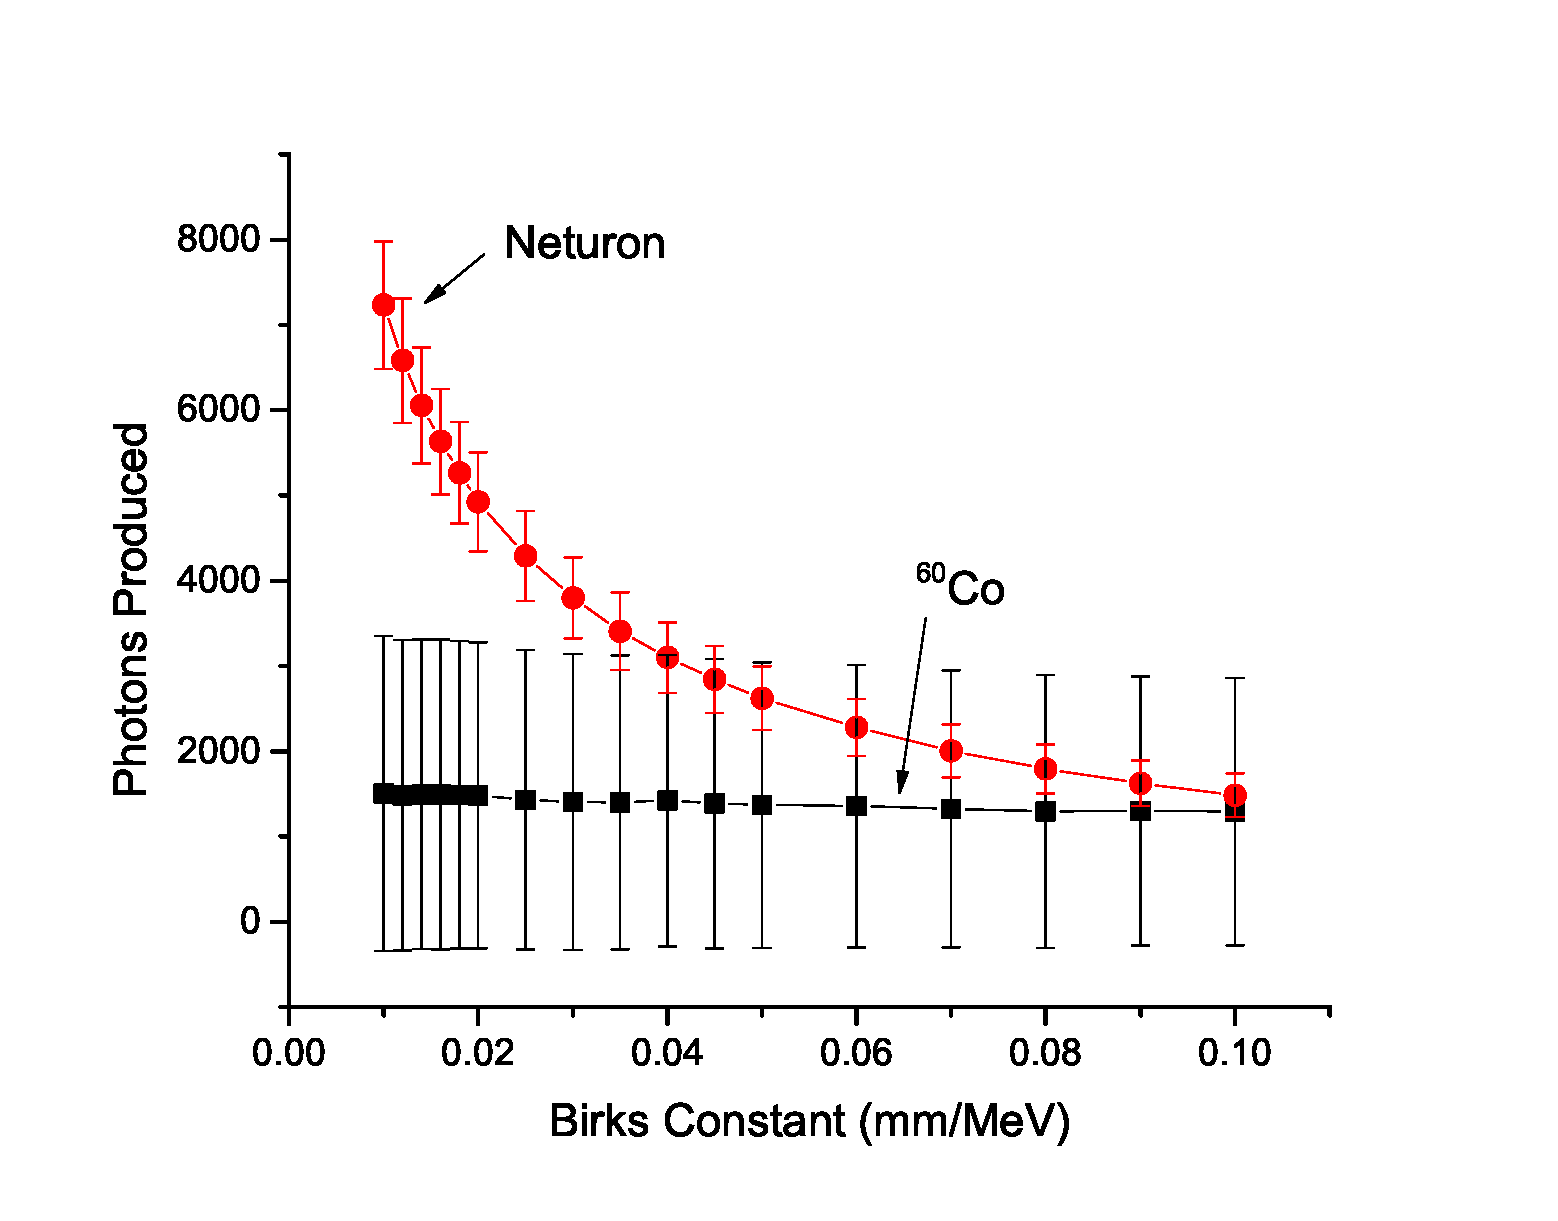
\includegraphics[width=\textwidth]{GS20_BirksVariation.eps}
	\caption{Simulated Gamma and Neutron Optical Photon production in GS20 for various Birks Constants.}
	\label{fig:GS20BirksVariation}
\end{figure}
\begin{figure}
	\centering
	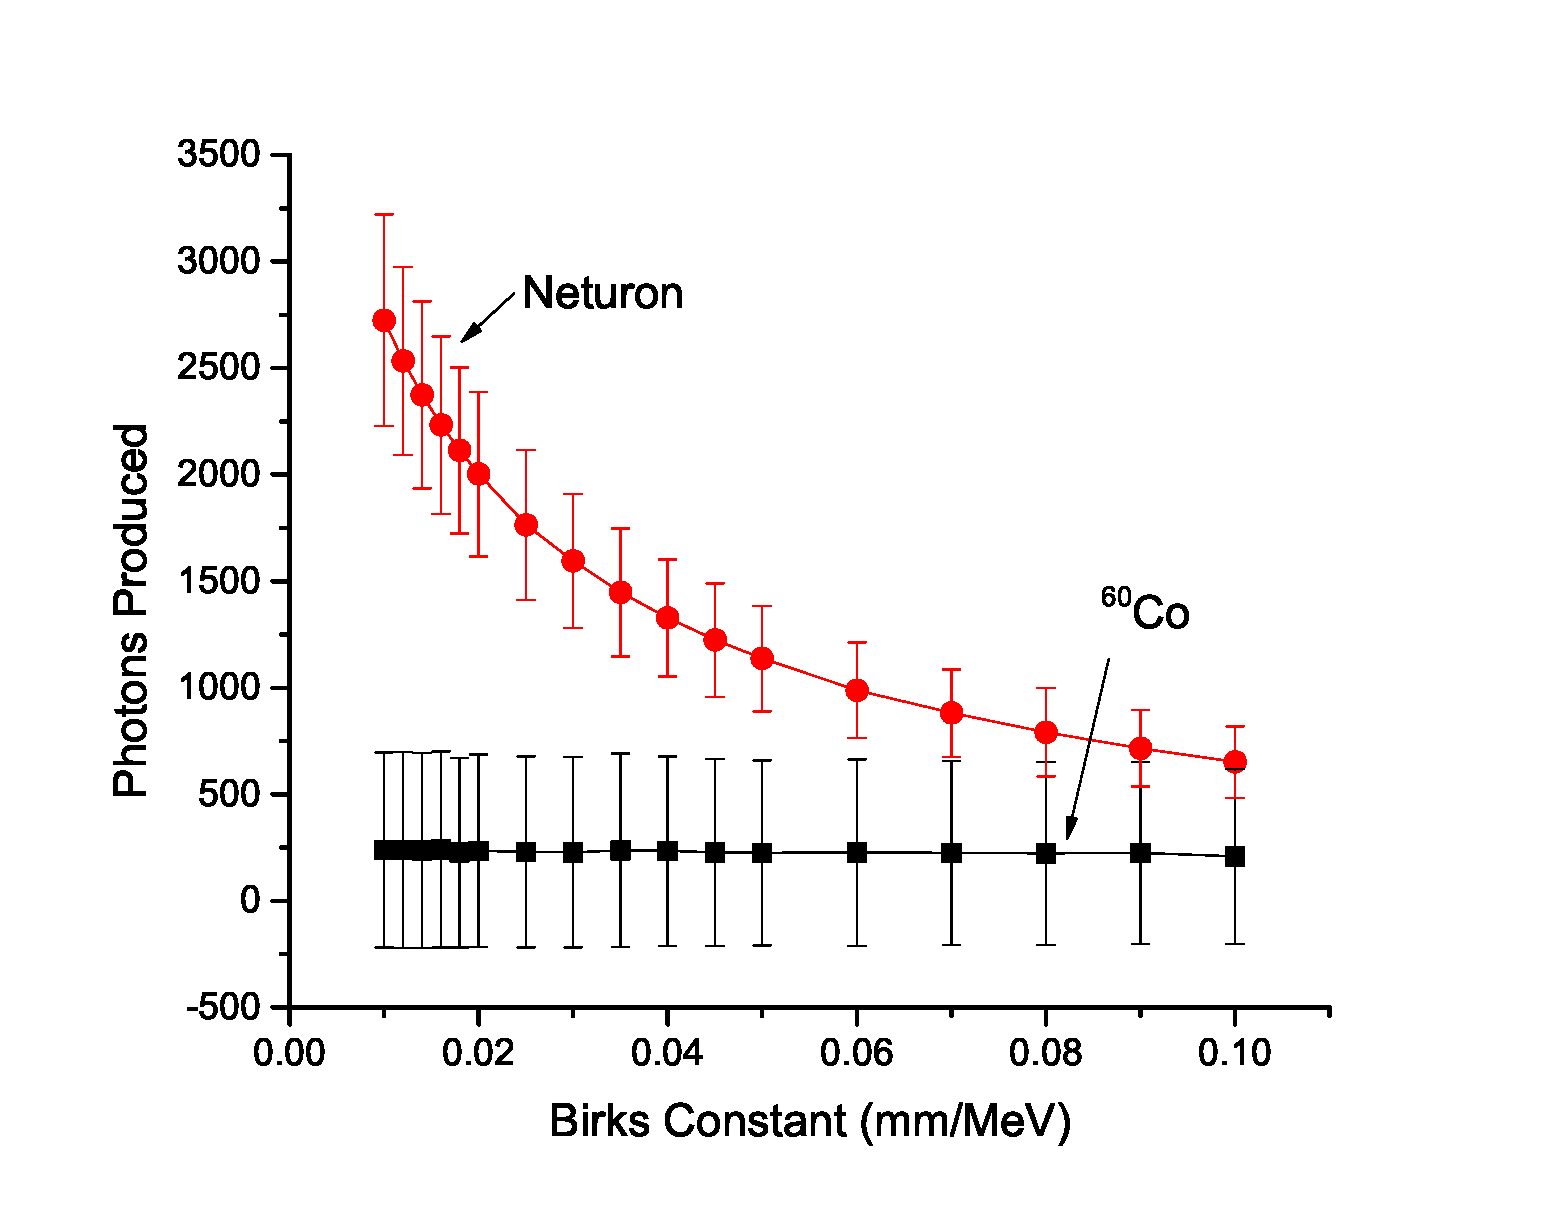
\includegraphics[width=\textwidth]{PSLiF_BirksVariation.eps}
	\caption[Simulated Gamma and Neutron Optical Photon Production in PS]{Simulated gamma and neutron optical photon production in polystyrene for various Birks Constants. A lower Birks constant indicates that a lower pulse height deficit.}
	\label{fig:PSBirksVariation}
\end{figure}

The resolution of the a detector can be set with the \verb+RESOLUTION+ parameter in the material property table.
The relationship between the \verb+RESOLUTION+ parameter and the FWMH can be described as \eqref{eqn:ScintResolution}
\begin{align}
	\label{eqn:ScintResolution}
	\text{RESOLUTION} = \frac{R}{2.35} \sqrt{E\times\text{SCINTILLATIONYIELD}}
\end{align}
where \definevar{$R$}{precent resolution (FWHM/Peak)} measured at the peak energy, $E$.
For GS20, where the precent resolution is around 15\%, this yields a \verb+RESOLUTION+ of eight.
